\documentclass[1p]{elsarticle_modified}
%\bibliographystyle{elsarticle-num}

%\usepackage[colorlinks]{hyperref}
%\usepackage{abbrmath_seonhwa} %\Abb, \Ascr, \Acal ,\Abf, \Afrak
\usepackage{amsfonts}
\usepackage{amssymb}
\usepackage{amsmath}
\usepackage{amsthm}
\usepackage{scalefnt}
\usepackage{amsbsy}
\usepackage{kotex}
\usepackage{caption}
\usepackage{subfig}
\usepackage{color}
\usepackage{graphicx}
\usepackage{xcolor} %% white, black, red, green, blue, cyan, magenta, yellow
\usepackage{float}
\usepackage{setspace}
\usepackage{hyperref}

\usepackage{tikz}
\usetikzlibrary{arrows}

\usepackage{multirow}
\usepackage{array} % fixed length table
\usepackage{hhline}

%%%%%%%%%%%%%%%%%%%%%
\makeatletter
\renewcommand*\env@matrix[1][\arraystretch]{%
	\edef\arraystretch{#1}%
	\hskip -\arraycolsep
	\let\@ifnextchar\new@ifnextchar
	\array{*\c@MaxMatrixCols c}}
\makeatother %https://tex.stackexchange.com/questions/14071/how-can-i-increase-the-line-spacing-in-a-matrix
%%%%%%%%%%%%%%%

\usepackage[normalem]{ulem}

\newcommand{\msout}[1]{\ifmmode\text{\sout{\ensuremath{#1}}}\else\sout{#1}\fi}
%SOURCE: \msout is \stkout macro in https://tex.stackexchange.com/questions/20609/strikeout-in-math-mode

\newcommand{\cancel}[1]{
	\ifmmode
	{\color{red}\msout{#1}}
	\else
	{\color{red}\sout{#1}}
	\fi
}

\newcommand{\add}[1]{
	{\color{blue}\uwave{#1}}
}

\newcommand{\replace}[2]{
	\ifmmode
	{\color{red}\msout{#1}}{\color{blue}\uwave{#2}}
	\else
	{\color{red}\sout{#1}}{\color{blue}\uwave{#2}}
	\fi
}

\newcommand{\Sol}{\mathcal{S}} %segment
\newcommand{\D}{D} %diagram
\newcommand{\A}{\mathcal{A}} %arc


%%%%%%%%%%%%%%%%%%%%%%%%%%%%%5 test

\def\sl{\operatorname{\textup{SL}}(2,\Cbb)}
\def\psl{\operatorname{\textup{PSL}}(2,\Cbb)}
\def\quan{\mkern 1mu \triangleright \mkern 1mu}

\theoremstyle{definition}
\newtheorem{thm}{Theorem}[section]
\newtheorem{prop}[thm]{Proposition}
\newtheorem{lem}[thm]{Lemma}
\newtheorem{ques}[thm]{Question}
\newtheorem{cor}[thm]{Corollary}
\newtheorem{defn}[thm]{Definition}
\newtheorem{exam}[thm]{Example}
\newtheorem{rmk}[thm]{Remark}
\newtheorem{alg}[thm]{Algorithm}

\newcommand{\I}{\sqrt{-1}}
\begin{document}

%\begin{frontmatter}
%
%\title{Boundary parabolic representations of knots up to 8 crossings}
%
%%% Group authors per affiliation:
%\author{Yunhi Cho} 
%\address{Department of Mathematics, University of Seoul, Seoul, Korea}
%\ead{yhcho@uos.ac.kr}
%
%
%\author{Seonhwa Kim} %\fnref{s_kim}}
%\address{Center for Geometry and Physics, Institute for Basic Science, Pohang, 37673, Korea}
%\ead{ryeona17@ibs.re.kr}
%
%\author{Hyuk Kim}
%\address{Department of Mathematical Sciences, Seoul National University, Seoul 08826, Korea}
%\ead{hyukkim@snu.ac.kr}
%
%\author{Seokbeom Yoon}
%\address{Department of Mathematical Sciences, Seoul National University, Seoul, 08826,  Korea}
%\ead{sbyoon15@snu.ac.kr}
%
%\begin{abstract}
%We find all boundary parabolic representation of knots up to 8 crossings.
%
%\end{abstract}
%\begin{keyword}
%    \MSC[2010] 57M25 
%\end{keyword}
%
%\end{frontmatter}

%\linenumbers
%\tableofcontents
%
\newcommand\colored[1]{\textcolor{white}{\rule[-0.35ex]{0.8em}{1.4ex}}\kern-0.8em\color{red} #1}%
%\newcommand\colored[1]{\textcolor{white}{ #1}\kern-2.17ex	\textcolor{white}{ #1}\kern-1.81ex	\textcolor{white}{ #1}\kern-2.15ex\color{red}#1	}

{\Large $\underline{12a_{0557}~(K12a_{0557})}$}

\setlength{\tabcolsep}{10pt}
\renewcommand{\arraystretch}{1.6}
\vspace{1cm}\begin{tabular}{m{100pt}>{\centering\arraybackslash}m{274pt}}
\multirow{5}{120pt}{
	\centering
	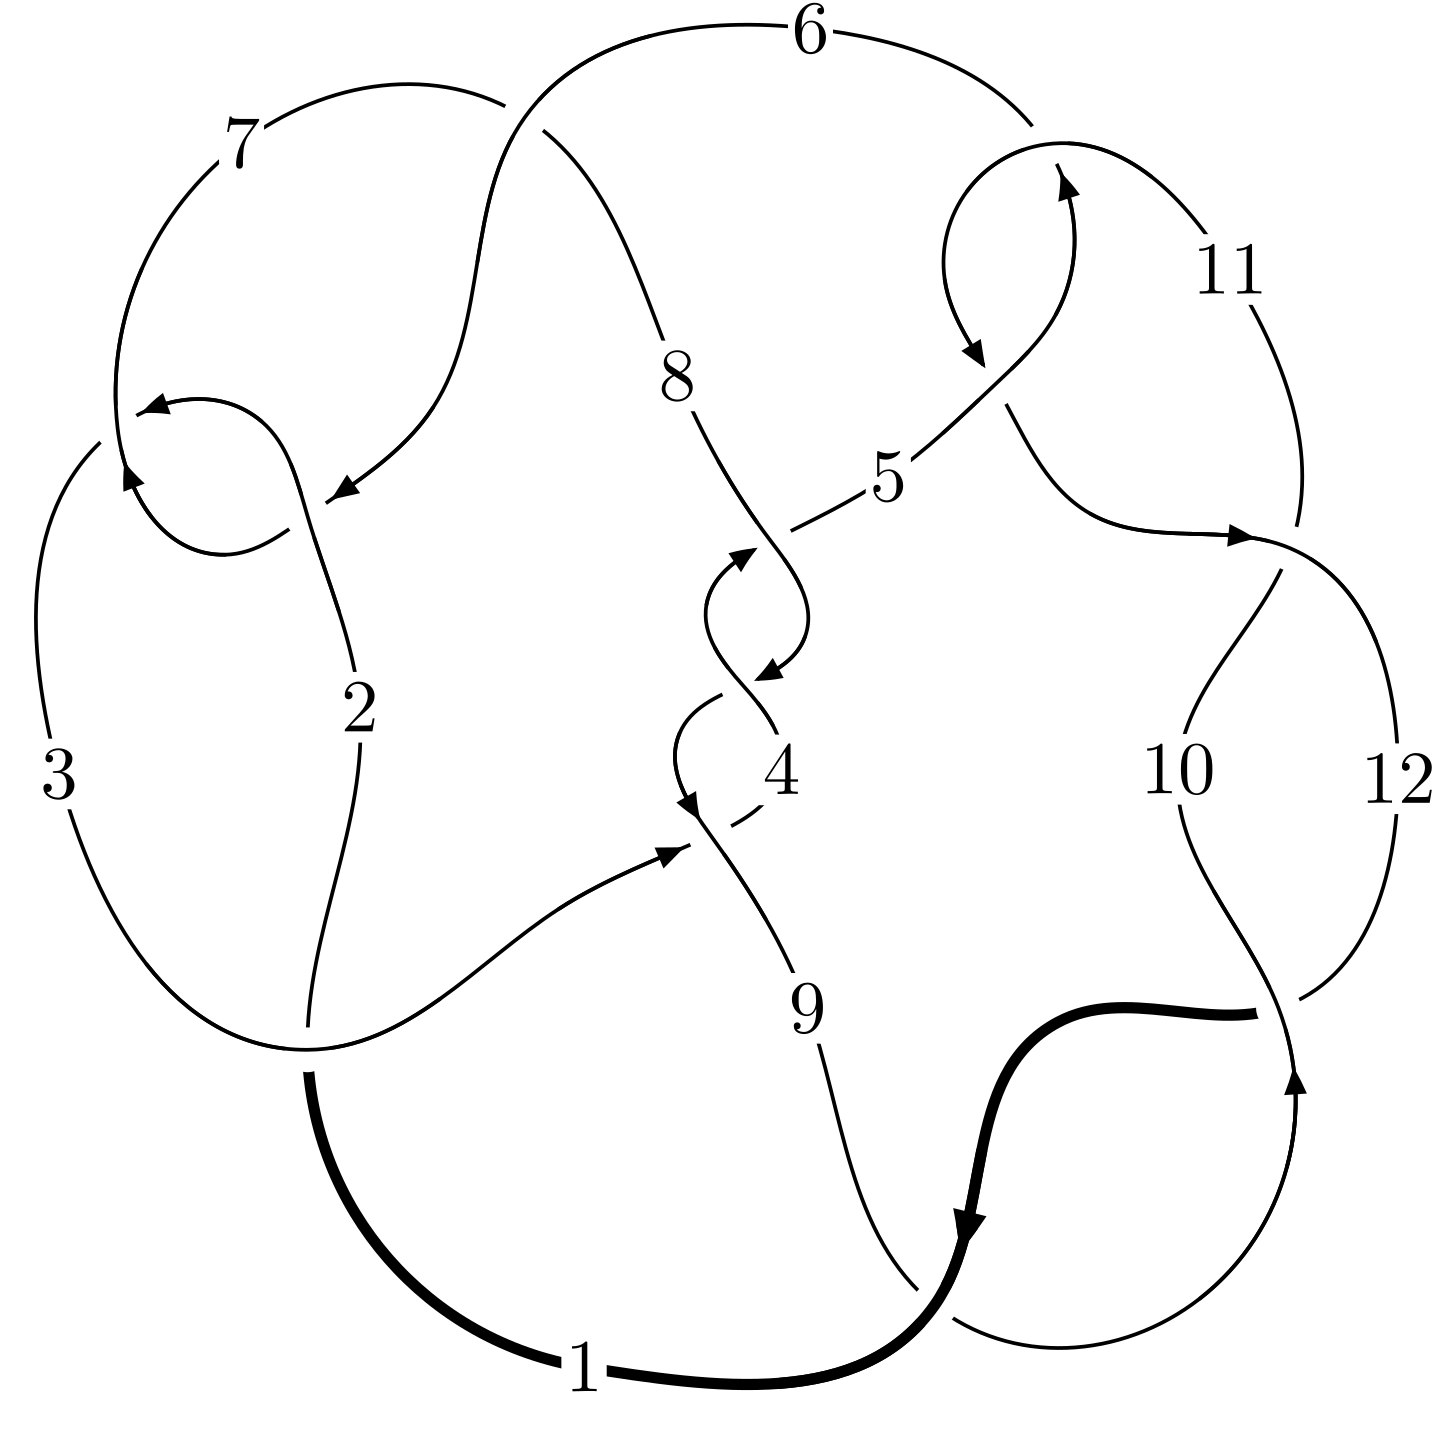
\includegraphics[width=112pt]{../../../GIT/diagram.site/Diagrams/png/1358_12a_0557.png}\\
\ \ \ A knot diagram\footnotemark}&
\allowdisplaybreaks
\textbf{Linearized knot diagam} \\
\cline{2-2}
 &
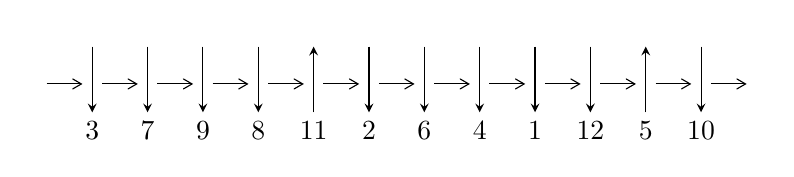
\begin{tikzpicture}[x=20pt, y=17pt]
	% nodes
	\node (C0) at (0, 0) {};
	\node (C1) at (1, 0) {};
	\node (C1U) at (1, +1) {};
	\node (C1D) at (1, -1) {3};

	\node (C2) at (2, 0) {};
	\node (C2U) at (2, +1) {};
	\node (C2D) at (2, -1) {7};

	\node (C3) at (3, 0) {};
	\node (C3U) at (3, +1) {};
	\node (C3D) at (3, -1) {9};

	\node (C4) at (4, 0) {};
	\node (C4U) at (4, +1) {};
	\node (C4D) at (4, -1) {8};

	\node (C5) at (5, 0) {};
	\node (C5U) at (5, +1) {};
	\node (C5D) at (5, -1) {11};

	\node (C6) at (6, 0) {};
	\node (C6U) at (6, +1) {};
	\node (C6D) at (6, -1) {2};

	\node (C7) at (7, 0) {};
	\node (C7U) at (7, +1) {};
	\node (C7D) at (7, -1) {6};

	\node (C8) at (8, 0) {};
	\node (C8U) at (8, +1) {};
	\node (C8D) at (8, -1) {4};

	\node (C9) at (9, 0) {};
	\node (C9U) at (9, +1) {};
	\node (C9D) at (9, -1) {1};

	\node (C10) at (10, 0) {};
	\node (C10U) at (10, +1) {};
	\node (C10D) at (10, -1) {12};

	\node (C11) at (11, 0) {};
	\node (C11U) at (11, +1) {};
	\node (C11D) at (11, -1) {5};

	\node (C12) at (12, 0) {};
	\node (C12U) at (12, +1) {};
	\node (C12D) at (12, -1) {10};
	\node (C13) at (13, 0) {};

	% arrows
	\draw[->,>={angle 60}]
	(C0) edge (C1) (C1) edge (C2) (C2) edge (C3) (C3) edge (C4) (C4) edge (C5) (C5) edge (C6) (C6) edge (C7) (C7) edge (C8) (C8) edge (C9) (C9) edge (C10) (C10) edge (C11) (C11) edge (C12) (C12) edge (C13) ;	\draw[->,>=stealth]
	(C1U) edge (C1D) (C2U) edge (C2D) (C3U) edge (C3D) (C4U) edge (C4D) (C5D) edge (C5U) (C6U) edge (C6D) (C7U) edge (C7D) (C8U) edge (C8D) (C9U) edge (C9D) (C10U) edge (C10D) (C11D) edge (C11U) (C12U) edge (C12D) ;
	\end{tikzpicture} \\
\hhline{~~} \\& 
\textbf{Solving Sequence} \\ \cline{2-2} 
 &
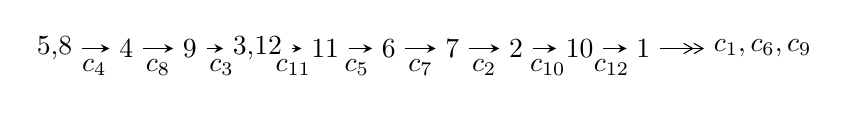
\begin{tikzpicture}[x=23pt, y=7pt]
	% node
	\node (A0) at (-1/8, 0) {5,8};
	\node (A1) at (1, 0) {4};
	\node (A2) at (2, 0) {9};
	\node (A3) at (49/16, 0) {3,12};
	\node (A4) at (33/8, 0) {11};
	\node (A5) at (41/8, 0) {6};
	\node (A6) at (49/8, 0) {7};
	\node (A7) at (57/8, 0) {2};
	\node (A8) at (65/8, 0) {10};
	\node (A9) at (73/8, 0) {1};
	\node (C1) at (1/2, -1) {$c_{4}$};
	\node (C2) at (3/2, -1) {$c_{8}$};
	\node (C3) at (5/2, -1) {$c_{3}$};
	\node (C4) at (29/8, -1) {$c_{11}$};
	\node (C5) at (37/8, -1) {$c_{5}$};
	\node (C6) at (45/8, -1) {$c_{7}$};
	\node (C7) at (53/8, -1) {$c_{2}$};
	\node (C8) at (61/8, -1) {$c_{10}$};
	\node (C9) at (69/8, -1) {$c_{12}$};
	\node (A10) at (11, 0) {$c_{1},c_{6},c_{9}$};

	% edge
	\draw[->,>=stealth]	
	(A0) edge (A1) (A1) edge (A2) (A2) edge (A3) (A3) edge (A4) (A4) edge (A5) (A5) edge (A6) (A6) edge (A7) (A7) edge (A8) (A8) edge (A9) ;
	\draw[->>,>={angle 60}]	
	(A9) edge (A10);
\end{tikzpicture} \\ 

\end{tabular} \\

\footnotetext{
The image of knot diagram is generated by the software ``\textbf{Draw programme}" developed by Andrew Bartholomew(\url{http://www.layer8.co.uk/maths/draw/index.htm\#Running-draw}), where we modified some parts for our purpose(\url{https://github.com/CATsTAILs/LinksPainter}).
}\phantom \\ \newline 
\centering \textbf{Ideals for irreducible components\footnotemark of $X_{\text{par}}$} 
 
\begin{align*}
I^u_{1}&=\langle 
1.49508\times10^{98} u^{64}+3.45396\times10^{98} u^{63}+\cdots+1.71880\times10^{101} b-6.24196\times10^{100},\\
\phantom{I^u_{1}}&\phantom{= \langle  }7.40968\times10^{98} u^{64}+4.71743\times10^{98} u^{63}+\cdots+1.56255\times10^{100} a+4.47963\times10^{99},\;u^{65}+u^{64}+\cdots-25 u-25\rangle \\
I^u_{2}&=\langle 
-13687 a^5 u-12349 a^4 u+\cdots-16925 a+1043,\\
\phantom{I^u_{2}}&\phantom{= \langle  }a^6+2 a^5 u- a^4 u-4 a^4-7 a^3 u+6 a^3+8 a^2 u+6 a^2-4 a u-11 a- u+6,\;u^2+1\rangle \\
\\
\end{align*}
\raggedright * 2 irreducible components of $\dim_{\mathbb{C}}=0$, with total 77 representations.\\
\footnotetext{All coefficients of polynomials are rational numbers. But the coefficients are sometimes approximated in decimal forms when there is not enough margin.}
\newpage
\renewcommand{\arraystretch}{1}
\centering \section*{I. $I^u_{1}= \langle 1.50\times10^{98} u^{64}+3.45\times10^{98} u^{63}+\cdots+1.72\times10^{101} b-6.24\times10^{100},\;7.41\times10^{98} u^{64}+4.72\times10^{98} u^{63}+\cdots+1.56\times10^{100} a+4.48\times10^{99},\;u^{65}+u^{64}+\cdots-25 u-25 \rangle$}
\flushleft \textbf{(i) Arc colorings}\\
\begin{tabular}{m{7pt} m{180pt} m{7pt} m{180pt} }
\flushright $a_{5}=$&$\begin{pmatrix}1\\0\end{pmatrix}$ \\
\flushright $a_{8}=$&$\begin{pmatrix}0\\u\end{pmatrix}$ \\
\flushright $a_{4}=$&$\begin{pmatrix}1\\- u^2\end{pmatrix}$ \\
\flushright $a_{9}=$&$\begin{pmatrix}- u\\u^3+u\end{pmatrix}$ \\
\flushright $a_{3}=$&$\begin{pmatrix}u^2+1\\- u^4-2 u^2\end{pmatrix}$ \\
\flushright $a_{12}=$&$\begin{pmatrix}-0.0474205 u^{64}-0.0301906 u^{63}+\cdots+7.10316 u-0.286687\\-0.000869840 u^{64}-0.00200952 u^{63}+\cdots-0.135624 u+0.363158\end{pmatrix}$ \\
\flushright $a_{11}=$&$\begin{pmatrix}-0.0465507 u^{64}-0.0281811 u^{63}+\cdots+7.23878 u-0.649845\\-0.000869840 u^{64}-0.00200952 u^{63}+\cdots-0.135624 u+0.363158\end{pmatrix}$ \\
\flushright $a_{6}=$&$\begin{pmatrix}0.0150022 u^{64}+0.0129683 u^{63}+\cdots+2.59978 u-2.71871\\-0.00372994 u^{64}-0.00195650 u^{63}+\cdots+1.02293 u+0.756420\end{pmatrix}$ \\
\flushright $a_{7}=$&$\begin{pmatrix}-0.0176087 u^{64}-0.0141154 u^{63}+\cdots+6.93497 u-1.17013\\-0.00433770 u^{64}-0.0109885 u^{63}+\cdots-0.534815 u+0.289329\end{pmatrix}$ \\
\flushright $a_{2}=$&$\begin{pmatrix}0.0346066 u^{64}+0.0170099 u^{63}+\cdots-6.02149 u+0.689262\\-0.00352626 u^{64}-0.00697665 u^{63}+\cdots+1.54019 u+0.392222\end{pmatrix}$ \\
\flushright $a_{10}=$&$\begin{pmatrix}-0.0317390 u^{64}-0.0250886 u^{63}+\cdots+1.23774 u-0.670406\\-0.00724756 u^{64}-0.0123758 u^{63}+\cdots+1.06301 u+0.201180\end{pmatrix}$ \\
\flushright $a_{1}=$&$\begin{pmatrix}-0.0299964 u^{64}-0.0121632 u^{63}+\cdots+3.39288 u-0.548318\\0.00192211 u^{64}-0.00142328 u^{63}+\cdots-1.37640 u-0.164022\end{pmatrix}$\\&\end{tabular}
\flushleft \textbf{(ii) Obstruction class $= -1$}\\~\\
\flushleft \textbf{(iii) Cusp Shapes $= 0.0739830 u^{64}+0.0434787 u^{63}+\cdots+8.13540 u-8.87805$}\\~\\
\newpage\renewcommand{\arraystretch}{1}
\flushleft \textbf{(iv) u-Polynomials at the component}\newline \\
\begin{tabular}{m{50pt}|m{274pt}}
Crossings & \hspace{64pt}u-Polynomials at each crossing \\
\hline $$\begin{aligned}c_{1},c_{7}\end{aligned}$$&$\begin{aligned}
&u^{65}+19 u^{64}+\cdots+5 u+1
\end{aligned}$\\
\hline $$\begin{aligned}c_{2},c_{6}\end{aligned}$$&$\begin{aligned}
&u^{65}- u^{64}+\cdots+3 u+1
\end{aligned}$\\
\hline $$\begin{aligned}c_{3},c_{4},c_{8}\end{aligned}$$&$\begin{aligned}
&u^{65}- u^{64}+\cdots-25 u+25
\end{aligned}$\\
\hline $$\begin{aligned}c_{5},c_{11}\end{aligned}$$&$\begin{aligned}
&u^{65}+u^{64}+\cdots-5 u+1
\end{aligned}$\\
\hline $$\begin{aligned}c_{9},c_{10},c_{12}\end{aligned}$$&$\begin{aligned}
&u^{65}+15 u^{64}+\cdots+7 u-1
\end{aligned}$\\
\hline
\end{tabular}\\~\\
\newpage\renewcommand{\arraystretch}{1}
\flushleft \textbf{(v) Riley Polynomials at the component}\newline \\
\begin{tabular}{m{50pt}|m{274pt}}
Crossings & \hspace{64pt}Riley Polynomials at each crossing \\
\hline $$\begin{aligned}c_{1},c_{7}\end{aligned}$$&$\begin{aligned}
&y^{65}+61 y^{64}+\cdots-107 y-1
\end{aligned}$\\
\hline $$\begin{aligned}c_{2},c_{6}\end{aligned}$$&$\begin{aligned}
&y^{65}-19 y^{64}+\cdots+5 y-1
\end{aligned}$\\
\hline $$\begin{aligned}c_{3},c_{4},c_{8}\end{aligned}$$&$\begin{aligned}
&y^{65}+71 y^{64}+\cdots-7625 y-625
\end{aligned}$\\
\hline $$\begin{aligned}c_{5},c_{11}\end{aligned}$$&$\begin{aligned}
&y^{65}+15 y^{64}+\cdots+7 y-1
\end{aligned}$\\
\hline $$\begin{aligned}c_{9},c_{10},c_{12}\end{aligned}$$&$\begin{aligned}
&y^{65}+75 y^{64}+\cdots-101 y-1
\end{aligned}$\\
\hline
\end{tabular}\\~\\
\newpage\flushleft \textbf{(vi) Complex Volumes and Cusp Shapes}
$$\begin{array}{c|c|c}  
\text{Solutions to }I^u_{1}& \I (\text{vol} + \sqrt{-1}CS) & \text{Cusp shape}\\
 \hline 
\begin{aligned}
u &= -0.194939 + 0.985568 I \\
a &= \phantom{-}1.136230 - 0.286521 I \\
b &= \phantom{-}0.757307 - 0.912410 I\end{aligned}
 & \phantom{-}4.66678 - 3.00289 I & -8.00000 + 0. I\phantom{ +0.000000I} \\ \hline\begin{aligned}
u &= -0.194939 - 0.985568 I \\
a &= \phantom{-}1.136230 + 0.286521 I \\
b &= \phantom{-}0.757307 + 0.912410 I\end{aligned}
 & \phantom{-}4.66678 + 3.00289 I & -8.00000 + 0. I\phantom{ +0.000000I} \\ \hline\begin{aligned}
u &= \phantom{-}0.143383 + 0.948907 I \\
a &= -0.264910 - 0.796535 I \\
b &= -0.235093 + 0.116598 I\end{aligned}
 & \phantom{-}1.78080 - 2.10362 I & \phantom{-0.000000 -}0. + 4.48623 I \\ \hline\begin{aligned}
u &= \phantom{-}0.143383 - 0.948907 I \\
a &= -0.264910 + 0.796535 I \\
b &= -0.235093 - 0.116598 I\end{aligned}
 & \phantom{-}1.78080 + 2.10362 I & \phantom{-0.000000 } 0. - 4.48623 I \\ \hline\begin{aligned}
u &= \phantom{-}0.221402 + 0.901501 I \\
a &= \phantom{-}1.47954 - 0.11084 I \\
b &= \phantom{-}0.781778 - 0.855158 I\end{aligned}
 & \phantom{-}4.84956 - 2.80174 I & -1.96434 + 4.08273 I \\ \hline\begin{aligned}
u &= \phantom{-}0.221402 - 0.901501 I \\
a &= \phantom{-}1.47954 + 0.11084 I \\
b &= \phantom{-}0.781778 + 0.855158 I\end{aligned}
 & \phantom{-}4.84956 + 2.80174 I & -1.96434 - 4.08273 I \\ \hline\begin{aligned}
u &= -0.444661 + 0.777234 I \\
a &= \phantom{-}0.408200 - 0.203744 I \\
b &= -0.506414 + 0.612963 I\end{aligned}
 & \phantom{-}2.38441 - 2.58306 I & -3.08948 + 3.45648 I \\ \hline\begin{aligned}
u &= -0.444661 - 0.777234 I \\
a &= \phantom{-}0.408200 + 0.203744 I \\
b &= -0.506414 - 0.612963 I\end{aligned}
 & \phantom{-}2.38441 + 2.58306 I & -3.08948 - 3.45648 I \\ \hline\begin{aligned}
u &= -0.200493 + 1.105690 I \\
a &= \phantom{-}0.077851 - 0.634026 I \\
b &= -0.156729 + 0.869731 I\end{aligned}
 & -0.456321 + 0.587854 I & \phantom{-0.000000 } 0 \\ \hline\begin{aligned}
u &= -0.200493 - 1.105690 I \\
a &= \phantom{-}0.077851 + 0.634026 I \\
b &= -0.156729 - 0.869731 I\end{aligned}
 & -0.456321 - 0.587854 I & \phantom{-0.000000 } 0\\
 \hline 
 \end{array}$$\newpage$$\begin{array}{c|c|c}  
\text{Solutions to }I^u_{1}& \I (\text{vol} + \sqrt{-1}CS) & \text{Cusp shape}\\
 \hline 
\begin{aligned}
u &= \phantom{-}0.540784 + 0.670619 I \\
a &= -0.252084 - 0.024836 I \\
b &= \phantom{-}0.558240 + 0.478764 I\end{aligned}
 & \phantom{-}2.54249 - 2.69464 I & -2.33919 + 3.35970 I \\ \hline\begin{aligned}
u &= \phantom{-}0.540784 - 0.670619 I \\
a &= -0.252084 + 0.024836 I \\
b &= \phantom{-}0.558240 - 0.478764 I\end{aligned}
 & \phantom{-}2.54249 + 2.69464 I & -2.33919 - 3.35970 I \\ \hline\begin{aligned}
u &= -0.991125 + 0.561749 I \\
a &= -1.220950 + 0.689343 I \\
b &= -0.863665 - 0.958398 I\end{aligned}
 & \phantom{-}9.74563 + 9.54545 I & \phantom{-0.000000 } 0 \\ \hline\begin{aligned}
u &= -0.991125 - 0.561749 I \\
a &= -1.220950 - 0.689343 I \\
b &= -0.863665 + 0.958398 I\end{aligned}
 & \phantom{-}9.74563 - 9.54545 I & \phantom{-0.000000 } 0 \\ \hline\begin{aligned}
u &= \phantom{-}0.973757 + 0.615749 I \\
a &= -0.383570 - 0.233418 I \\
b &= -0.896873 - 0.885529 I\end{aligned}
 & \phantom{-}9.97887 - 3.03863 I & \phantom{-0.000000 } 0 \\ \hline\begin{aligned}
u &= \phantom{-}0.973757 - 0.615749 I \\
a &= -0.383570 + 0.233418 I \\
b &= -0.896873 + 0.885529 I\end{aligned}
 & \phantom{-}9.97887 + 3.03863 I & \phantom{-0.000000 } 0 \\ \hline\begin{aligned}
u &= \phantom{-}0.947294 + 0.674719 I \\
a &= \phantom{-}1.243340 + 0.582206 I \\
b &= \phantom{-}0.874408 - 0.938153 I\end{aligned}
 & \phantom{-}10.15870 - 3.31862 I & \phantom{-0.000000 } 0 \\ \hline\begin{aligned}
u &= \phantom{-}0.947294 - 0.674719 I \\
a &= \phantom{-}1.243340 - 0.582206 I \\
b &= \phantom{-}0.874408 + 0.938153 I\end{aligned}
 & \phantom{-}10.15870 + 3.31862 I & \phantom{-0.000000 } 0 \\ \hline\begin{aligned}
u &= -0.925321 + 0.731778 I \\
a &= \phantom{-}0.465765 - 0.237270 I \\
b &= \phantom{-}0.887478 - 0.908982 I\end{aligned}
 & \phantom{-}10.25190 - 3.19464 I & \phantom{-0.000000 } 0 \\ \hline\begin{aligned}
u &= -0.925321 - 0.731778 I \\
a &= \phantom{-}0.465765 + 0.237270 I \\
b &= \phantom{-}0.887478 + 0.908982 I\end{aligned}
 & \phantom{-}10.25190 + 3.19464 I & \phantom{-0.000000 } 0\\
 \hline 
 \end{array}$$\newpage$$\begin{array}{c|c|c}  
\text{Solutions to }I^u_{1}& \I (\text{vol} + \sqrt{-1}CS) & \text{Cusp shape}\\
 \hline 
\begin{aligned}
u &= -0.666201 + 0.415426 I \\
a &= \phantom{-}0.53075 - 1.62998 I \\
b &= \phantom{-}0.470202 + 0.892585 I\end{aligned}
 & \phantom{-}1.24733 + 6.64277 I & -7.43550 - 9.53298 I \\ \hline\begin{aligned}
u &= -0.666201 - 0.415426 I \\
a &= \phantom{-}0.53075 + 1.62998 I \\
b &= \phantom{-}0.470202 - 0.892585 I\end{aligned}
 & \phantom{-}1.24733 - 6.64277 I & -7.43550 + 9.53298 I \\ \hline\begin{aligned}
u &= -0.037730 + 1.240550 I \\
a &= -1.51164 - 0.80363 I \\
b &= -0.426053 - 0.548434 I\end{aligned}
 & \phantom{-}2.00616 - 1.49123 I & \phantom{-0.000000 } 0 \\ \hline\begin{aligned}
u &= -0.037730 - 1.240550 I \\
a &= -1.51164 + 0.80363 I \\
b &= -0.426053 + 0.548434 I\end{aligned}
 & \phantom{-}2.00616 + 1.49123 I & \phantom{-0.000000 } 0 \\ \hline\begin{aligned}
u &= \phantom{-}0.117997 + 1.274100 I \\
a &= \phantom{-}1.40404 - 0.21152 I \\
b &= \phantom{-}0.612078 - 0.723737 I\end{aligned}
 & \phantom{-}4.41355 - 2.28333 I & \phantom{-0.000000 } 0 \\ \hline\begin{aligned}
u &= \phantom{-}0.117997 - 1.274100 I \\
a &= \phantom{-}1.40404 + 0.21152 I \\
b &= \phantom{-}0.612078 + 0.723737 I\end{aligned}
 & \phantom{-}4.41355 + 2.28333 I & \phantom{-0.000000 } 0 \\ \hline\begin{aligned}
u &= \phantom{-}0.574683 + 0.420836 I \\
a &= -0.34710 - 1.45942 I \\
b &= -0.499917 + 0.810111 I\end{aligned}
 & \phantom{-}1.75044 - 1.32012 I & -5.66585 + 3.92029 I \\ \hline\begin{aligned}
u &= \phantom{-}0.574683 - 0.420836 I \\
a &= -0.34710 + 1.45942 I \\
b &= -0.499917 - 0.810111 I\end{aligned}
 & \phantom{-}1.75044 + 1.32012 I & -5.66585 - 3.92029 I \\ \hline\begin{aligned}
u &= -0.165173 + 1.283860 I \\
a &= -1.78999 + 0.19957 I \\
b &= -0.424688 - 0.860379 I\end{aligned}
 & \phantom{-}0.95184 + 4.92361 I & \phantom{-0.000000 } 0 \\ \hline\begin{aligned}
u &= -0.165173 - 1.283860 I \\
a &= -1.78999 - 0.19957 I \\
b &= -0.424688 + 0.860379 I\end{aligned}
 & \phantom{-}0.95184 - 4.92361 I & \phantom{-0.000000 } 0\\
 \hline 
 \end{array}$$\newpage$$\begin{array}{c|c|c}  
\text{Solutions to }I^u_{1}& \I (\text{vol} + \sqrt{-1}CS) & \text{Cusp shape}\\
 \hline 
\begin{aligned}
u &= -0.572720 + 0.106229 I \\
a &= \phantom{-}0.96365 - 1.74351 I \\
b &= \phantom{-}0.262020 + 0.873062 I\end{aligned}
 & -3.34907 + 2.30473 I & -16.2162 - 5.9449 I \\ \hline\begin{aligned}
u &= -0.572720 - 0.106229 I \\
a &= \phantom{-}0.96365 + 1.74351 I \\
b &= \phantom{-}0.262020 - 0.873062 I\end{aligned}
 & -3.34907 - 2.30473 I & -16.2162 + 5.9449 I \\ \hline\begin{aligned}
u &= -0.437487 + 0.332448 I \\
a &= -2.32984 + 0.82322 I \\
b &= -0.784409 - 0.913662 I\end{aligned}
 & \phantom{-}2.66558 + 5.57488 I & -9.42845 - 7.52087 I \\ \hline\begin{aligned}
u &= -0.437487 - 0.332448 I \\
a &= -2.32984 - 0.82322 I \\
b &= -0.784409 + 0.913662 I\end{aligned}
 & \phantom{-}2.66558 - 5.57488 I & -9.42845 + 7.52087 I \\ \hline\begin{aligned}
u &= -0.04732 + 1.49280 I \\
a &= \phantom{-}0.003876 - 0.697847 I \\
b &= -0.024391 + 1.094580 I\end{aligned}
 & \phantom{-}4.94320 + 3.00427 I & \phantom{-0.000000 } 0 \\ \hline\begin{aligned}
u &= -0.04732 - 1.49280 I \\
a &= \phantom{-}0.003876 + 0.697847 I \\
b &= -0.024391 - 1.094580 I\end{aligned}
 & \phantom{-}4.94320 - 3.00427 I & \phantom{-0.000000 } 0 \\ \hline\begin{aligned}
u &= -0.13405 + 1.51695 I \\
a &= \phantom{-}2.18073 + 0.49322 I \\
b &= \phantom{-}0.859141 + 0.947236 I\end{aligned}
 & \phantom{-}8.98795 + 7.60409 I & \phantom{-0.000000 } 0 \\ \hline\begin{aligned}
u &= -0.13405 - 1.51695 I \\
a &= \phantom{-}2.18073 - 0.49322 I \\
b &= \phantom{-}0.859141 - 0.947236 I\end{aligned}
 & \phantom{-}8.98795 - 7.60409 I & \phantom{-0.000000 } 0 \\ \hline\begin{aligned}
u &= \phantom{-}0.09167 + 1.52042 I \\
a &= \phantom{-}1.60247 + 1.13624 I \\
b &= \phantom{-}0.883757 + 0.890653 I\end{aligned}
 & \phantom{-}9.16830 - 1.15187 I & \phantom{-0.000000 } 0 \\ \hline\begin{aligned}
u &= \phantom{-}0.09167 - 1.52042 I \\
a &= \phantom{-}1.60247 - 1.13624 I \\
b &= \phantom{-}0.883757 - 0.890653 I\end{aligned}
 & \phantom{-}9.16830 + 1.15187 I & \phantom{-0.000000 } 0\\
 \hline 
 \end{array}$$\newpage$$\begin{array}{c|c|c}  
\text{Solutions to }I^u_{1}& \I (\text{vol} + \sqrt{-1}CS) & \text{Cusp shape}\\
 \hline 
\begin{aligned}
u &= \phantom{-}0.353629 + 0.307016 I \\
a &= -0.21266 - 1.52151 I \\
b &= -0.789122 - 0.859153 I\end{aligned}
 & \phantom{-}2.82730 + 0.34334 I & -9.08497 + 2.02539 I \\ \hline\begin{aligned}
u &= \phantom{-}0.353629 - 0.307016 I \\
a &= -0.21266 + 1.52151 I \\
b &= -0.789122 + 0.859153 I\end{aligned}
 & \phantom{-}2.82730 - 0.34334 I & -9.08497 - 2.02539 I \\ \hline\begin{aligned}
u &= \phantom{-}0.13146 + 1.52657 I \\
a &= \phantom{-}1.221890 + 0.412179 I \\
b &= \phantom{-}0.516210 - 1.047730 I\end{aligned}
 & \phantom{-}8.27904 - 3.65206 I & \phantom{-0.000000 } 0 \\ \hline\begin{aligned}
u &= \phantom{-}0.13146 - 1.52657 I \\
a &= \phantom{-}1.221890 - 0.412179 I \\
b &= \phantom{-}0.516210 + 1.047730 I\end{aligned}
 & \phantom{-}8.27904 + 3.65206 I & \phantom{-0.000000 } 0 \\ \hline\begin{aligned}
u &= -0.21085 + 1.52413 I \\
a &= -1.252790 + 0.515874 I \\
b &= -0.473206 - 1.059010 I\end{aligned}
 & \phantom{-}7.69875 + 9.80033 I & \phantom{-0.000000 } 0 \\ \hline\begin{aligned}
u &= -0.21085 - 1.52413 I \\
a &= -1.252790 - 0.515874 I \\
b &= -0.473206 + 1.059010 I\end{aligned}
 & \phantom{-}7.69875 - 9.80033 I & \phantom{-0.000000 } 0 \\ \hline\begin{aligned}
u &= \phantom{-}0.455205\phantom{ +0.000000I} \\
a &= -0.0293311\phantom{ +0.000000I} \\
b &= \phantom{-}0.404527\phantom{ +0.000000I}\end{aligned}
 & -1.07813\phantom{ +0.000000I} & -9.13920\phantom{ +0.000000I} \\ \hline\begin{aligned}
u &= \phantom{-}0.14198 + 1.58601 I \\
a &= -0.829734 - 0.378431 I \\
b &= -0.825125 - 0.320393 I\end{aligned}
 & \phantom{-}10.16130 - 5.11867 I & \phantom{-0.000000 } 0 \\ \hline\begin{aligned}
u &= \phantom{-}0.14198 - 1.58601 I \\
a &= -0.829734 + 0.378431 I \\
b &= -0.825125 + 0.320393 I\end{aligned}
 & \phantom{-}10.16130 + 5.11867 I & \phantom{-0.000000 } 0 \\ \hline\begin{aligned}
u &= -0.05580 + 1.59350 I \\
a &= \phantom{-}0.883115 - 0.344042 I \\
b &= \phantom{-}0.829266 - 0.381772 I\end{aligned}
 & \phantom{-}10.48610 - 1.22570 I & \phantom{-0.000000 } 0\\
 \hline 
 \end{array}$$\newpage$$\begin{array}{c|c|c}  
\text{Solutions to }I^u_{1}& \I (\text{vol} + \sqrt{-1}CS) & \text{Cusp shape}\\
 \hline 
\begin{aligned}
u &= -0.05580 - 1.59350 I \\
a &= \phantom{-}0.883115 + 0.344042 I \\
b &= \phantom{-}0.829266 + 0.381772 I\end{aligned}
 & \phantom{-}10.48610 + 1.22570 I & \phantom{-0.000000 } 0 \\ \hline\begin{aligned}
u &= \phantom{-}0.265152 + 0.297533 I \\
a &= -1.128460 - 0.499441 I \\
b &= -0.222502 + 0.644711 I\end{aligned}
 & -0.359965 - 0.971629 I & -6.26553 + 6.85953 I \\ \hline\begin{aligned}
u &= \phantom{-}0.265152 - 0.297533 I \\
a &= -1.128460 + 0.499441 I \\
b &= -0.222502 - 0.644711 I\end{aligned}
 & -0.359965 + 0.971629 I & -6.26553 - 6.85953 I \\ \hline\begin{aligned}
u &= \phantom{-}0.02254 + 1.60792 I \\
a &= -1.73396 + 0.67808 I \\
b &= -0.893399 + 0.929362 I\end{aligned}
 & \phantom{-}13.28270 - 3.29649 I & \phantom{-0.000000 } 0 \\ \hline\begin{aligned}
u &= \phantom{-}0.02254 - 1.60792 I \\
a &= -1.73396 - 0.67808 I \\
b &= -0.893399 - 0.929362 I\end{aligned}
 & \phantom{-}13.28270 + 3.29649 I & \phantom{-0.000000 } 0 \\ \hline\begin{aligned}
u &= -0.35667 + 1.60371 I \\
a &= \phantom{-}1.91240 - 0.16841 I \\
b &= \phantom{-}0.857112 + 1.009490 I\end{aligned}
 & \phantom{-}16.7892 + 14.5383 I & \phantom{-0.000000 } 0 \\ \hline\begin{aligned}
u &= -0.35667 - 1.60371 I \\
a &= \phantom{-}1.91240 + 0.16841 I \\
b &= \phantom{-}0.857112 - 1.009490 I\end{aligned}
 & \phantom{-}16.7892 - 14.5383 I & \phantom{-0.000000 } 0 \\ \hline\begin{aligned}
u &= \phantom{-}0.33299 + 1.62729 I \\
a &= \phantom{-}0.916394 + 0.913504 I \\
b &= \phantom{-}0.942347 + 0.840020 I\end{aligned}
 & \phantom{-}17.3369 - 7.9187 I & \phantom{-0.000000 } 0 \\ \hline\begin{aligned}
u &= \phantom{-}0.33299 - 1.62729 I \\
a &= \phantom{-}0.916394 - 0.913504 I \\
b &= \phantom{-}0.942347 - 0.840020 I\end{aligned}
 & \phantom{-}17.3369 + 7.9187 I & \phantom{-0.000000 } 0 \\ \hline\begin{aligned}
u &= \phantom{-}0.30253 + 1.64433 I \\
a &= -1.84849 - 0.02882 I \\
b &= -0.872298 + 1.000890 I\end{aligned}
 & \phantom{-}17.8412 - 8.0089 I & \phantom{-0.000000 } 0\\
 \hline 
 \end{array}$$\newpage$$\begin{array}{c|c|c}  
\text{Solutions to }I^u_{1}& \I (\text{vol} + \sqrt{-1}CS) & \text{Cusp shape}\\
 \hline 
\begin{aligned}
u &= \phantom{-}0.30253 - 1.64433 I \\
a &= -1.84849 + 0.02882 I \\
b &= -0.872298 - 1.000890 I\end{aligned}
 & \phantom{-}17.8412 + 8.0089 I & \phantom{-0.000000 } 0 \\ \hline\begin{aligned}
u &= -0.27148 + 1.66645 I \\
a &= -1.042730 + 0.849827 I \\
b &= -0.944098 + 0.861611 I\end{aligned}
 & \phantom{-}18.2931 + 1.3306 I & \phantom{-0.000000 } 0 \\ \hline\begin{aligned}
u &= -0.27148 - 1.66645 I \\
a &= -1.042730 - 0.849827 I \\
b &= -0.944098 - 0.861611 I\end{aligned}
 & \phantom{-}18.2931 - 1.3306 I & \phantom{-0.000000 } 0 \\ \hline\begin{aligned}
u &= -0.176841 + 0.243173 I \\
a &= \phantom{-}1.23332 + 4.42124 I \\
b &= \phantom{-}0.044375 - 0.853831 I\end{aligned}
 & -1.05566 + 2.24342 I & -14.4833 - 3.3091 I \\ \hline\begin{aligned}
u &= -0.176841 - 0.243173 I \\
a &= \phantom{-}1.23332 - 4.42124 I \\
b &= \phantom{-}0.044375 + 0.853831 I\end{aligned}
 & -1.05566 - 2.24342 I & -14.4833 + 3.3091 I\\
 \hline 
 \end{array}$$\newpage\newpage\renewcommand{\arraystretch}{1}
\centering \section*{II. $I^u_{2}= \langle -13687 a^5 u-12349 a^4 u+\cdots-16925 a+1043,\;2 a^5 u- a^4 u+\cdots-11 a+6,\;u^2+1 \rangle$}
\flushleft \textbf{(i) Arc colorings}\\
\begin{tabular}{m{7pt} m{180pt} m{7pt} m{180pt} }
\flushright $a_{5}=$&$\begin{pmatrix}1\\0\end{pmatrix}$ \\
\flushright $a_{8}=$&$\begin{pmatrix}0\\u\end{pmatrix}$ \\
\flushright $a_{4}=$&$\begin{pmatrix}1\\1\end{pmatrix}$ \\
\flushright $a_{9}=$&$\begin{pmatrix}- u\\0\end{pmatrix}$ \\
\flushright $a_{3}=$&$\begin{pmatrix}0\\1\end{pmatrix}$ \\
\flushright $a_{12}=$&$\begin{pmatrix}a\\0.184498 a^{5} u+0.166462 a^{4} u+\cdots+0.228146 a-0.0140594\end{pmatrix}$ \\
\flushright $a_{11}=$&$\begin{pmatrix}-0.184498 a^{5} u-0.166462 a^{4} u+\cdots+0.771854 a+0.0140594\\0.184498 a^{5} u+0.166462 a^{4} u+\cdots+0.228146 a-0.0140594\end{pmatrix}$ \\
\flushright $a_{6}=$&$\begin{pmatrix}0.0408978 a^{5} u+0.129177 a^{4} u+\cdots+0.154613 a+0.806484\\-0.167972 a^{5} u-0.213143 a^{4} u+\cdots+0.380805 a+0.496178\end{pmatrix}$ \\
\flushright $a_{7}=$&$\begin{pmatrix}0.0408978 a^{5} u+0.129177 a^{4} u+\cdots+0.154613 a+0.806484\\-0.182126 a^{5} u-0.0785469 a^{4} u+\cdots+0.763025 a-0.786224\end{pmatrix}$ \\
\flushright $a_{2}=$&$\begin{pmatrix}0.0179551 a^{5} u-0.0164589 a^{4} u+\cdots+0.0922693 a+0.329676\\-0.0874301 a^{5} u+0.282847 a^{4} u+\cdots+1.08674 a-1.08730\end{pmatrix}$ \\
\flushright $a_{10}=$&$\begin{pmatrix}-0.182126 a^{5} u-0.0785469 a^{4} u+\cdots+0.763025 a-0.786224\\0.0791130 a^{5} u+0.465768 a^{4} u+\cdots+1.22262 a-1.43103\end{pmatrix}$ \\
\flushright $a_{1}=$&$\begin{pmatrix}0.0179551 a^{5} u-0.0164589 a^{4} u+\cdots+0.0922693 a+0.329676\\-0.105385 a^{5} u+0.299306 a^{4} u+\cdots+0.994473 a-1.41697\end{pmatrix}$\\&\end{tabular}
\flushleft \textbf{(ii) Obstruction class $= 1$}\\~\\
\flushleft \textbf{(iii) Cusp Shapes $= \frac{11172}{74185} a^5 u-\frac{66884}{74185} a^5-\frac{88436}{74185} a^4 u-\frac{87728}{74185} a^4-\frac{10956}{14837} a^3 u+\frac{31104}{14837} a^3+\frac{61696}{14837} a^2 u-\frac{7576}{14837} a^2+\frac{22716}{14837} a u-\frac{73396}{14837} a+\frac{235144}{74185} u-\frac{192528}{74185}$}\\~\\
\newpage\renewcommand{\arraystretch}{1}
\flushleft \textbf{(iv) u-Polynomials at the component}\newline \\
\begin{tabular}{m{50pt}|m{274pt}}
Crossings & \hspace{64pt}u-Polynomials at each crossing \\
\hline $$\begin{aligned}c_{1}\end{aligned}$$&$\begin{aligned}
&(u^2- u+1)^6
\end{aligned}$\\
\hline $$\begin{aligned}c_{2},c_{6}\end{aligned}$$&$\begin{aligned}
&(u^4- u^2+1)^3
\end{aligned}$\\
\hline $$\begin{aligned}c_{3},c_{4},c_{8}\end{aligned}$$&$\begin{aligned}
&(u^2+1)^6
\end{aligned}$\\
\hline $$\begin{aligned}c_{5},c_{11}\end{aligned}$$&$\begin{aligned}
&(u^6+u^4+2 u^2+1)^2
\end{aligned}$\\
\hline $$\begin{aligned}c_{7}\end{aligned}$$&$\begin{aligned}
&(u^2+u+1)^6
\end{aligned}$\\
\hline $$\begin{aligned}c_{9},c_{10}\end{aligned}$$&$\begin{aligned}
&(u^3- u^2+2 u-1)^4
\end{aligned}$\\
\hline $$\begin{aligned}c_{12}\end{aligned}$$&$\begin{aligned}
&(u^3+u^2+2 u+1)^4
\end{aligned}$\\
\hline
\end{tabular}\\~\\
\newpage\renewcommand{\arraystretch}{1}
\flushleft \textbf{(v) Riley Polynomials at the component}\newline \\
\begin{tabular}{m{50pt}|m{274pt}}
Crossings & \hspace{64pt}Riley Polynomials at each crossing \\
\hline $$\begin{aligned}c_{1},c_{7}\end{aligned}$$&$\begin{aligned}
&(y^2+y+1)^6
\end{aligned}$\\
\hline $$\begin{aligned}c_{2},c_{6}\end{aligned}$$&$\begin{aligned}
&(y^2- y+1)^6
\end{aligned}$\\
\hline $$\begin{aligned}c_{3},c_{4},c_{8}\end{aligned}$$&$\begin{aligned}
&(y+1)^{12}
\end{aligned}$\\
\hline $$\begin{aligned}c_{5},c_{11}\end{aligned}$$&$\begin{aligned}
&(y^3+y^2+2 y+1)^4
\end{aligned}$\\
\hline $$\begin{aligned}c_{9},c_{10},c_{12}\end{aligned}$$&$\begin{aligned}
&(y^3+3 y^2+2 y-1)^4
\end{aligned}$\\
\hline
\end{tabular}\\~\\
\newpage\flushleft \textbf{(vi) Complex Volumes and Cusp Shapes}
$$\begin{array}{c|c|c}  
\text{Solutions to }I^u_{2}& \I (\text{vol} + \sqrt{-1}CS) & \text{Cusp shape}\\
 \hline 
\begin{aligned}
u &= \phantom{-0.000000 -}1.000000 I \\
a &= \phantom{-}0.662359 + 0.577399 I \\
b &= \phantom{-0.000000 -}0.754878 I\end{aligned}
 & \phantom{-}0.53148 - 2.02988 I & -9.01951 + 3.46410 I \\ \hline\begin{aligned}
u &= \phantom{-0.000000 -}1.000000 I \\
a &= \phantom{-}0.489013 - 0.507560 I \\
b &= \phantom{-}0.744862 - 0.877439 I\end{aligned}
 & \phantom{-}4.66906 - 4.85801 I & -2.49024 + 6.44355 I \\ \hline\begin{aligned}
u &= \phantom{-0.000000 -}1.000000 I \\
a &= -1.15137 - 1.06984 I \\
b &= -0.744862 - 0.877439 I\end{aligned}
 & \phantom{-}4.66906 + 0.79824 I & -2.49024 + 0.48465 I \\ \hline\begin{aligned}
u &= \phantom{-0.000000 -}1.000000 I \\
a &= \phantom{-}1.46291 + 0.63968 I \\
b &= \phantom{-}0.744862 - 0.877439 I\end{aligned}
 & \phantom{-}4.66906 - 0.79824 I & -2.49024 - 0.48465 I \\ \hline\begin{aligned}
u &= \phantom{-0.000000 -}1.000000 I \\
a &= \phantom{-}0.66236 - 1.71708 I \\
b &= \phantom{-0.000000 -}0.754878 I\end{aligned}
 & \phantom{-}0.53148 + 2.02988 I & -9.01951 - 3.46410 I \\ \hline\begin{aligned}
u &= \phantom{-0.000000 -}1.000000 I \\
a &= -2.12527 + 0.07740 I \\
b &= -0.744862 - 0.877439 I\end{aligned}
 & \phantom{-}4.66906 + 4.85801 I & -2.49024 - 6.44355 I \\ \hline\begin{aligned}
u &= \phantom{-0.000000 } -1.000000 I \\
a &= \phantom{-}0.662359 - 0.577399 I \\
b &= \phantom{-0.000000 } -0.754878 I\end{aligned}
 & \phantom{-}0.53148 + 2.02988 I & -9.01951 - 3.46410 I \\ \hline\begin{aligned}
u &= \phantom{-0.000000 } -1.000000 I \\
a &= \phantom{-}0.489013 + 0.507560 I \\
b &= \phantom{-}0.744862 + 0.877439 I\end{aligned}
 & \phantom{-}4.66906 + 4.85801 I & -2.49024 - 6.44355 I \\ \hline\begin{aligned}
u &= \phantom{-0.000000 } -1.000000 I \\
a &= -1.15137 + 1.06984 I \\
b &= -0.744862 + 0.877439 I\end{aligned}
 & \phantom{-}4.66906 - 0.79824 I & -2.49024 - 0.48465 I \\ \hline\begin{aligned}
u &= \phantom{-0.000000 } -1.000000 I \\
a &= \phantom{-}1.46291 - 0.63968 I \\
b &= \phantom{-}0.744862 + 0.877439 I\end{aligned}
 & \phantom{-}4.66906 + 0.79824 I & -2.49024 + 0.48465 I\\
 \hline 
 \end{array}$$\newpage$$\begin{array}{c|c|c}  
\text{Solutions to }I^u_{2}& \I (\text{vol} + \sqrt{-1}CS) & \text{Cusp shape}\\
 \hline 
\begin{aligned}
u &= \phantom{-0.000000 } -1.000000 I \\
a &= \phantom{-}0.66236 + 1.71708 I \\
b &= \phantom{-0.000000 } -0.754878 I\end{aligned}
 & \phantom{-}0.53148 - 2.02988 I & -9.01951 + 3.46410 I \\ \hline\begin{aligned}
u &= \phantom{-0.000000 } -1.000000 I \\
a &= -2.12527 - 0.07740 I \\
b &= -0.744862 + 0.877439 I\end{aligned}
 & \phantom{-}4.66906 - 4.85801 I & -2.49024 + 6.44355 I\\
 \hline 
 \end{array}$$\newpage
\newpage\renewcommand{\arraystretch}{1}
\centering \section*{ III. u-Polynomials}
\begin{tabular}{m{50pt}|m{274pt}}
Crossings & \hspace{64pt}u-Polynomials at each crossing \\
\hline $$\begin{aligned}c_{1}\end{aligned}$$&$\begin{aligned}
&((u^2- u+1)^6)(u^{65}+19 u^{64}+\cdots+5 u+1)
\end{aligned}$\\
\hline $$\begin{aligned}c_{2},c_{6}\end{aligned}$$&$\begin{aligned}
&((u^4- u^2+1)^3)(u^{65}- u^{64}+\cdots+3 u+1)
\end{aligned}$\\
\hline $$\begin{aligned}c_{3},c_{4},c_{8}\end{aligned}$$&$\begin{aligned}
&((u^2+1)^6)(u^{65}- u^{64}+\cdots-25 u+25)
\end{aligned}$\\
\hline $$\begin{aligned}c_{5},c_{11}\end{aligned}$$&$\begin{aligned}
&((u^6+u^4+2 u^2+1)^2)(u^{65}+u^{64}+\cdots-5 u+1)
\end{aligned}$\\
\hline $$\begin{aligned}c_{7}\end{aligned}$$&$\begin{aligned}
&((u^2+u+1)^6)(u^{65}+19 u^{64}+\cdots+5 u+1)
\end{aligned}$\\
\hline $$\begin{aligned}c_{9},c_{10}\end{aligned}$$&$\begin{aligned}
&((u^3- u^2+2 u-1)^4)(u^{65}+15 u^{64}+\cdots+7 u-1)
\end{aligned}$\\
\hline $$\begin{aligned}c_{12}\end{aligned}$$&$\begin{aligned}
&((u^3+u^2+2 u+1)^4)(u^{65}+15 u^{64}+\cdots+7 u-1)
\end{aligned}$\\
\hline
\end{tabular}\newpage\renewcommand{\arraystretch}{1}
\centering \section*{ IV. Riley Polynomials}
\begin{tabular}{m{50pt}|m{274pt}}
Crossings & \hspace{64pt}Riley Polynomials at each crossing \\
\hline $$\begin{aligned}c_{1},c_{7}\end{aligned}$$&$\begin{aligned}
&((y^2+y+1)^6)(y^{65}+61 y^{64}+\cdots-107 y-1)
\end{aligned}$\\
\hline $$\begin{aligned}c_{2},c_{6}\end{aligned}$$&$\begin{aligned}
&((y^2- y+1)^6)(y^{65}-19 y^{64}+\cdots+5 y-1)
\end{aligned}$\\
\hline $$\begin{aligned}c_{3},c_{4},c_{8}\end{aligned}$$&$\begin{aligned}
&((y+1)^{12})(y^{65}+71 y^{64}+\cdots-7625 y-625)
\end{aligned}$\\
\hline $$\begin{aligned}c_{5},c_{11}\end{aligned}$$&$\begin{aligned}
&((y^3+y^2+2 y+1)^4)(y^{65}+15 y^{64}+\cdots+7 y-1)
\end{aligned}$\\
\hline $$\begin{aligned}c_{9},c_{10},c_{12}\end{aligned}$$&$\begin{aligned}
&((y^3+3 y^2+2 y-1)^4)(y^{65}+75 y^{64}+\cdots-101 y-1)
\end{aligned}$\\
\hline
\end{tabular}
\vskip 2pc
\end{document}